\chapter{継承}
\label{chap:inheritance}

この章では、クラスをもとにして別のクラスを作る「継承」について学びます。第11章では、\texttt{Ball}クラスや\texttt{FallingSquare}クラスを作り、フィールド、コンストラクタ、メソッド、インスタンスの考え方を学びました。

円を落とすクラスと正方形を落とすクラスを見比べると、位置、速さ、画面外に出たときの処理など、よく似た部分がたくさんあります。継承は、このような「似ているクラス」を整理し、共通する部分を1か所にまとめるための仕組みです。

\section{この章の概要}

この章では、点を少しずつ揺らすクラスをもとに、正方形を表示するクラスへ拡張する例を通して、継承の考え方を学びます。

この章で扱う主な内容は次の通りです。

\begin{itemize}
    \item 似たクラスに共通する部分を見つける
    \item 親クラスと子クラス
    \item \texttt{extends}による継承
    \item \texttt{super}による親クラスのコンストラクタ呼び出し
    \item 子クラスでメソッドを上書きする方法
    \item 親クラス型の配列で子クラスをまとめる
    \item 第11章の落ちる図形への応用
\end{itemize}

\section{第11章からのつながり}

第11章では、円を表す\texttt{Ball}クラスを作り、その後で正方形を表す\texttt{FallingSquare}クラスも作りました。円と正方形は見た目こそ違いますが、どちらも「位置を持つ」「下に動く」「画面の下に出たら上に戻る」という点ではよく似ています。

\begin{center}
\begin{tabular}{lll}
\toprule
処理や情報 & 円のクラス & 正方形のクラス \\
\midrule
中心のx座標 & 必要 & 必要 \\
中心のy座標 & 必要 & 必要 \\
下向きの速さ & 必要 & 必要 \\
色 & 必要 & 必要 \\
画面外に出たら戻る処理 & 必要 & 必要 \\
描画方法 & 円を描く & 正方形を描く \\
\bottomrule
\end{tabular}
\end{center}

この表を見ると、違いは主に「どの図形を描くか」です。つまり、動き方は共通で、描き方だけが違うと考えられます。このようなときに継承を使うと、共通する動き方を親クラスにまとめ、描き方だけを子クラスで変えられます。

\begin{notebox}{継承は重複を減らすための道具}
継承は「コードを短くする魔法」ではありません。似ているクラスの共通部分を1か所にまとめ、違う部分だけを子クラスに書くための道具です。
\end{notebox}

\section{まずは揺れる点を作る}

まず、少しずつランダムに動く点を作ります。ここでは、最初に\texttt{JitteringDot}クラスを作ります。\texttt{jitter}は「小刻みに揺れる」という意味です。

\begin{listing}[htbp]
\inputminted{ts}{listings/chapter14/jittering-dot.ts}
\caption{少しずつランダムに動く点}
\label{lst:chapter14-jittering-dot}
\end{listing}

\texttt{JitteringDot}は、\texttt{centerX}と\texttt{centerY}を持ちます。\texttt{update}メソッドでは座標を少しだけ変え、\texttt{display}メソッドでは点を描きます。\texttt{p.constrain}は、値を指定した範囲の中におさめる関数です。

\begin{pointbox}{動きと見た目を分けて考える}
\texttt{update}は位置を変える処理、\texttt{display}は画面に描く処理です。この2つを分けておくと、あとで「動きは同じで見た目だけ違うもの」を作りやすくなります。
\end{pointbox}

\section{継承を使わずに正方形へ作り替える}

点ではなく正方形を揺らしたい場合、継承を使わずに別のクラスを作ることもできます。次のサンプルでは、\texttt{JitteringSquare}クラスを最初から作っています。

\begin{listing}[htbp]
\inputminted{ts}{listings/chapter14/jittering-square-without-inheritance.ts}
\caption{継承を使わずに揺れる正方形を作る}
\label{lst:chapter14-jittering-square-without-inheritance}
\end{listing}

このクラスは正方形を描けますが、\texttt{centerX}、\texttt{centerY}、\texttt{update}の中身が\texttt{JitteringDot}とほとんど同じです。もし移動の範囲や速さを変えたくなったら、点のクラスと正方形のクラスの両方を直す必要があります。

\begin{mistakebox}{コピーして少し変えるだけでは増えるほど大変になる}
似たクラスをコピーして作ると、最初は簡単に見えます。しかし、同じ処理が複数の場所に増えるため、あとで修正するときに直し忘れが起きやすくなります。
\end{mistakebox}

\section{\texttt{extends}でクラスを拡張する}

継承を使うと、あるクラスをもとにして新しいクラスを作れます。もとになるクラスを親クラス、そこから作る新しいクラスを子クラスと呼びます。TypeScriptでは、\texttt{class 子クラス extends 親クラス}のように書きます。

\begin{figure}[htbp]
    \centering
    \begin{tikzpicture}[
        box/.style={rectangle, draw, rounded corners, minimum width=45mm, minimum height=12mm, align=center},
        arrow/.style={->, thick}
    ]
        \node[box, fill=blue!5] (parent) at (0, 0)
            {\texttt{JitteringDot}\\座標と\texttt{update}を持つ};
        \node[box, fill=green!5] (child) at (0, -1.8)
            {\texttt{JitteringSquare}\\一辺の長さと描き方を追加};
        \draw[arrow] (child.north) -- (parent.south);
        \node[align=center] at (3.5, -0.9) {\texttt{extends}\\親クラスをもとにする};
    \end{tikzpicture}
    \caption{親クラスと子クラスの関係}
    \label{fig:chapter14-parent-child}
\end{figure}

次のサンプルでは、\texttt{JitteringSquare}が\texttt{JitteringDot}を継承しています。正方形も点と同じように座標を持ち、\texttt{update}メソッドを使えます。

\begin{listing}[htbp]
\inputminted[firstline=1,lastline=25]{ts}{listings/chapter14/jittering-square-inheritance.ts}
\caption{親クラスになる\texttt{JitteringDot}}
\label{lst:chapter14-jittering-square-inheritance-parent}
\end{listing}

\begin{listing}[htbp]
\inputminted[firstline=27,lastline=43]{ts}{listings/chapter14/jittering-square-inheritance.ts}
\caption{\texttt{JitteringDot}を継承する\texttt{JitteringSquare}}
\label{lst:chapter14-jittering-square-inheritance-child}
\end{listing}

\begin{listing}[htbp]
\inputminted[firstline=45,lastline=61]{ts}{listings/chapter14/jittering-square-inheritance.ts}
\caption{継承したクラスを使うスケッチ}
\label{lst:chapter14-jittering-square-inheritance-sketch}
\end{listing}

\texttt{JitteringSquare extends JitteringDot}と書くことで、\texttt{JitteringSquare}は\texttt{JitteringDot}のフィールドとメソッドを引き継ぎます。そのため、\texttt{JitteringSquare}の中には\texttt{update}を書いていませんが、\texttt{square.update(p)}を呼び出せます。

\begin{pointbox}{子クラスは親クラスの機能を使える}
\texttt{JitteringSquare}には\texttt{update}メソッドを書いていません。それでも、親クラスの\texttt{JitteringDot}が\texttt{update}を持っているため、子クラスのインスタンスから呼び出せます。
\end{pointbox}

\section{\texttt{super}で親クラスのコンストラクタを呼ぶ}

子クラスのコンストラクタでは、まず親クラスのコンストラクタを呼び出します。そのために使うのが\texttt{super}です。サンプルでは、\texttt{super(centerX, centerY);}と書いて、親クラスの\texttt{JitteringDot}にx座標とy座標を渡しています。

\begin{center}
\begin{tabular}{ll}
\toprule
書き方 & 意味 \\
\midrule
\texttt{extends JitteringDot} & \texttt{JitteringDot}をもとにして作る \\
\texttt{super(centerX, centerY);} & 親クラスのコンストラクタを呼ぶ \\
\texttt{this.sideLength = sideLength;} & 子クラスで追加したフィールドに代入する \\
\bottomrule
\end{tabular}
\end{center}

\texttt{centerX}と\texttt{centerY}は親クラスが持つフィールドです。一方、\texttt{sideLength}は正方形だけが必要とするフィールドです。そのため、共通する初期化は\texttt{super}に任せ、正方形だけの初期化は子クラスの中に書きます。

\begin{mistakebox}{\texttt{super}を呼ぶ前に\texttt{this}を使わない}
子クラスのコンストラクタでは、\texttt{this.sideLength = ...}の前に\texttt{super(...)}を呼びます。親クラスの初期化が終わる前に\texttt{this}を使おうとするとエラーになります。
\end{mistakebox}

\section{メソッドを上書きする}

子クラスでは、親クラスと同じ名前、同じ形式のメソッドを書くことで、処理を上書きできます。ここでいう同じ形式とは、引数の数と型、戻り値の型をそろえることです。このことをメソッドの上書きと呼びます。上書きしたメソッドを呼ぶと、子クラスに書いた動作が実行されます。

\texttt{JitteringDot}の\texttt{display}は点を描きます。一方、\texttt{JitteringSquare}の\texttt{display}は正方形を描きます。どちらもメソッド名は\texttt{display}ですが、インスタンスの種類によって実行される中身が変わります。

\section{親クラス型の配列にまとめる}

継承の便利な点の1つは、親クラス型の配列に、子クラスのインスタンスも入れられることです。次のサンプルでは、\texttt{JitteringDot[]}の配列に、\texttt{JitteringDot}と\texttt{JitteringSquare}を一緒に入れています。

\begin{listing}[htbp]
\inputminted[firstline=1,lastline=43]{ts}{listings/chapter14/jittering-mixed-array.ts}
\caption{点と正方形で共通する親クラス}
\label{lst:chapter14-jittering-mixed-array-classes}
\end{listing}

\begin{listing}[htbp]
\inputminted[firstline=45,lastline=67]{ts}{listings/chapter14/jittering-mixed-array.ts}
\caption{親クラス型の配列でまとめて動かす}
\label{lst:chapter14-jittering-mixed-array-sketch}
\end{listing}

\texttt{things}は\texttt{JitteringDot[]}型です。その中に\texttt{new JitteringSquare(...)}を入れられるのは、\texttt{JitteringSquare}が\texttt{JitteringDot}を継承しているからです。

\begin{pointbox}{同じ呼び方で違う描き方をする}
\texttt{things[index].display(p)}と同じ呼び方をしても、点のインスタンスなら点が描かれ、正方形のインスタンスなら正方形が描かれます。これが継承を使ったときの大きな利点です。
\end{pointbox}

\section{落ちる図形に継承を使う}

第11章の\texttt{Ball}と\texttt{FallingSquare}のような落ちる図形にも、継承を使えます。ここでは、共通する「落ちる動き」を\texttt{FallingShape}クラスにまとめ、円と正方形の描き方だけを子クラスで変えます。

\begin{listing}[htbp]
\inputminted[firstline=1,lastline=36]{ts}{listings/chapter14/falling-shapes-inheritance.ts}
\caption{落ちる図形の共通部分を表す\texttt{FallingShape}}
\label{lst:chapter14-falling-shape-parent}
\end{listing}

\begin{listing}[htbp]
\inputminted[firstline=38,lastline=53]{ts}{listings/chapter14/falling-shapes-inheritance.ts}
\caption{円と正方形の子クラス}
\label{lst:chapter14-falling-shape-children}
\end{listing}

\begin{listing}[htbp]
\inputminted[firstline=55,lastline=84]{ts}{listings/chapter14/falling-shapes-inheritance.ts}
\caption{落ちる円と正方形をまとめて動かす}
\label{lst:chapter14-falling-shape-sketch}
\end{listing}

\texttt{FallingShape}には、位置、大きさ、速さ、色、\texttt{update}メソッドがあります。\texttt{FallingCircle}と\texttt{FallingSquare}は、どちらも\texttt{FallingShape}を継承し、\texttt{display}だけをそれぞれの図形に合わせて書き換えています。

\begin{notebox}{親クラスにも\texttt{display}を書く理由}
\texttt{FallingShape[]}の配列に入れたものへ\texttt{shapes[index].display(p)}と書くため、親クラスにも\texttt{display}メソッドを用意しています。子クラスでは、その\texttt{display}を自分の描き方に上書きしています。
\end{notebox}

\section{共通メソッドを子クラスで使う}

親クラスが持っているメソッドは、子クラスのインスタンスでも使えます。次のサンプルでは、\texttt{isMouseOver}を親クラスに書き、丸い図形と正方形の両方で利用しています。

\begin{listing}[htbp]
\inputminted[firstline=1,lastline=43]{ts}{listings/chapter14/clickable-shapes.ts}
\caption{マウス判定を持つ親クラスと正方形の子クラス}
\label{lst:chapter14-clickable-shapes-classes}
\end{listing}

\begin{listing}[htbp]
\inputminted[firstline=45,lastline=71]{ts}{listings/chapter14/clickable-shapes.ts}
\caption{共通のマウス判定を使うスケッチ}
\label{lst:chapter14-clickable-shapes-sketch}
\end{listing}

\texttt{ClickableSquare}には\texttt{isMouseOver}を書いていません。それでも、親クラスの\texttt{ClickableShape}が\texttt{isMouseOver}を持っているため、\texttt{shapes[index].isMouseOver(p)}を呼び出せます。

\section{RPG風のキャラクターで考える}

ゲームを作るときにも、継承で考えやすい場面があります。たとえばRPGのようなゲームでは、主人公、魔法使い、騎士、モンスターなどが登場します。見た目や行動は違いますが、どのキャラクターも名前、HP、画面上の座標を持つ、と考えられます。

\begin{figure}[htbp]
    \centering
    \resizebox{\linewidth}{!}{%
    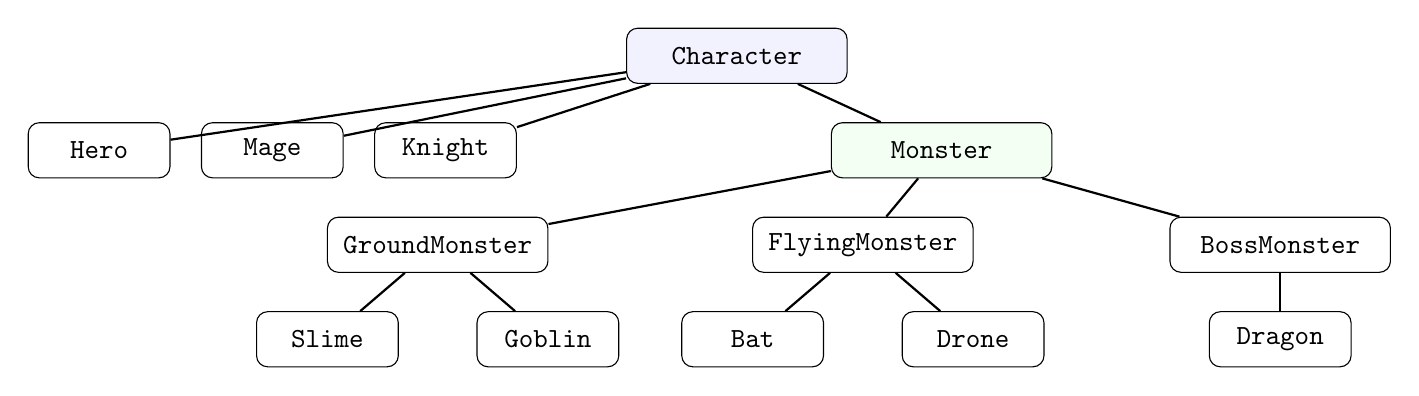
\begin{tikzpicture}[
        rpgNode/.style={rectangle, draw, rounded corners, align=center, minimum width=28mm, minimum height=7mm},
        rpgLeafNode/.style={rectangle, draw, rounded corners, align=center, minimum width=18mm, minimum height=7mm},
        line/.style={thick}
    ]
        \node[rpgNode, fill=blue!5] (character) at (0, 0) {\texttt{Character}};
        \node[rpgLeafNode] (hero) at (-8.1, -1.2) {\texttt{Hero}};
        \node[rpgLeafNode] (mage) at (-5.9, -1.2) {\texttt{Mage}};
        \node[rpgLeafNode] (knight) at (-3.7, -1.2) {\texttt{Knight}};
        \node[rpgNode, fill=green!5] (monster) at (2.6, -1.2) {\texttt{Monster}};
        \node[rpgNode] (ground) at (-3.8, -2.4) {\texttt{GroundMonster}};
        \node[rpgNode] (flying) at (1.6, -2.4) {\texttt{FlyingMonster}};
        \node[rpgNode] (boss) at (6.9, -2.4) {\texttt{BossMonster}};
        \node[rpgLeafNode] (slime) at (-5.2, -3.6) {\texttt{Slime}};
        \node[rpgLeafNode] (goblin) at (-2.4, -3.6) {\texttt{Goblin}};
        \node[rpgLeafNode] (bat) at (0.2, -3.6) {\texttt{Bat}};
        \node[rpgLeafNode] (drone) at (3.0, -3.6) {\texttt{Drone}};
        \node[rpgLeafNode] (dragon) at (6.9, -3.6) {\texttt{Dragon}};

        \draw[line] (character) -- (hero);
        \draw[line] (character) -- (mage);
        \draw[line] (character) -- (knight);
        \draw[line] (character) -- (monster);
        \draw[line] (monster) -- (ground);
        \draw[line] (monster) -- (flying);
        \draw[line] (monster) -- (boss);
        \draw[line] (ground) -- (slime);
        \draw[line] (ground) -- (goblin);
        \draw[line] (flying) -- (bat);
        \draw[line] (flying) -- (drone);
        \draw[line] (boss) -- (dragon);
    \end{tikzpicture}
    }
    \caption{RPG風キャラクターの継承関係}
    \label{fig:chapter14-rpg-inheritance-tree}
\end{figure}

この例では、\texttt{Character}に共通の情報を持たせます。そこから、味方キャラクターやモンスターを表す子クラスを作ります。\texttt{attack}、\texttt{magic}、\texttt{heal}は同じ名前のメソッドとして用意し、クラスごとに中身を変えます。

\begin{listing}[htbp]
\inputminted[firstline=1,lastline=45]{ts}{listings/chapter14/rpg-characters.ts}
\caption{共通部分を持つ\texttt{Character}クラス}
\label{lst:chapter14-rpg-character-base}
\end{listing}

\begin{listing}[htbp]
\inputminted[firstline=48,lastline=78]{ts}{listings/chapter14/rpg-characters.ts}
\caption{味方キャラクターと基本のモンスター}
\label{lst:chapter14-rpg-hero-monster}
\end{listing}

\begin{listing}[htbp]
\inputminted[firstline=80,lastline=114]{ts}{listings/chapter14/rpg-characters.ts}
\caption{地上と空中で分かれるモンスター}
\label{lst:chapter14-rpg-ground-flying-monsters}
\end{listing}

\begin{listing}[htbp]
\inputminted[firstline=116,lastline=130]{ts}{listings/chapter14/rpg-characters.ts}
\caption{ボスモンスターとドラゴン}
\label{lst:chapter14-rpg-boss-monster}
\end{listing}

\begin{listing}[htbp]
\inputminted[firstline=132,lastline=179]{ts}{listings/chapter14/rpg-characters.ts}
\caption{RPG風キャラクターを画面に表示する}
\label{lst:chapter14-rpg-sketch}
\end{listing}

\texttt{characters}は\texttt{Character[]}型の配列です。その中に\texttt{Hero}、\texttt{Mage}、\texttt{Knight}、\texttt{Slime}、\texttt{Dragon}などをまとめて入れています。どのクラスも\texttt{Character}をもとにしているため、同じ配列に入れられます。

\begin{pointbox}{共通の型でまとめ、違う行動を呼び出す}
\texttt{characters[0].attack()}と\texttt{characters[7].attack()}は同じ名前のメソッド呼び出しです。しかし、\texttt{Hero}なら剣で攻撃し、\texttt{Dragon}なら炎の息を吐きます。同じ呼び方で、インスタンスごとに違う行動をさせられるのが継承の面白いところです。
\end{pointbox}

\section{継承を使いすぎない}

継承は便利ですが、何でも継承にすればよいわけではありません。共通部分がはっきりしていて、「子クラスは親クラスの一種である」と自然に言えるときに使うと分かりやすくなります。

\begin{center}
\begin{tabular}{ll}
\toprule
考え方 & 例 \\
\midrule
使いやすい継承 & \texttt{FallingCircle}は\texttt{FallingShape}の一種 \\
分かりにくい継承 & \texttt{Player}は\texttt{Score}の一種 \\
\bottomrule
\end{tabular}
\end{center}

共通する処理が少ない場合や、親子関係として読むと不自然な場合は、無理に継承を使わなくてもかまいません。第11章のように別々のクラスとして書いた方が読みやすいこともあります。

\begin{notebox}{継承は設計の選択肢の1つ}
継承は、似たクラスを整理するための選択肢です。必ず使うものではありません。初学者の段階では、「共通部分を親クラスに置く」「違う部分を子クラスに置く」と読める場合に使う、くらいで十分です。
\end{notebox}

\begin{notebox}{\texttt{draw}という名前を避ける}
p5.jsの\texttt{p.draw}と区別しやすいように、図形クラスの描画メソッドは\texttt{display}と名付けます。
\end{notebox}

\section{よくある間違い}

継承では、親クラスと子クラスのどちらに何を書くのかが重要です。エラーが出たときは、\texttt{extends}の向き、\texttt{super}の呼び出し、メソッド名の一致を確認しましょう。

\begin{mistakebox}{\texttt{extends}の向きを逆にする}
\texttt{class JitteringSquare extends JitteringDot}は、「\texttt{JitteringSquare}は\texttt{JitteringDot}をもとにする」という意味です。親クラスと子クラスの順番を逆にしないようにしましょう。
\end{mistakebox}

\begin{mistakebox}{\texttt{super}を書き忘れる}
子クラスにコンストラクタを書く場合、基本的には最初に\texttt{super(...)}を呼びます。親クラスが持つフィールドの初期化を忘れないためです。
\end{mistakebox}

\begin{mistakebox}{メソッド名を少しだけ変えてしまう}
親クラスの\texttt{display}を上書きしたいのに、子クラスで\texttt{drawDisplay}のような別名を書いてしまうと、上書きにはなりません。同じ名前、同じ使い方で書くことを確認しましょう。
\end{mistakebox}

\begin{mistakebox}{親クラスにないメソッドを親クラス型の配列から呼ぶ}
\texttt{FallingShape[]}の配列から呼べるのは、\texttt{FallingShape}に定義されているメソッドです。子クラスだけが持つ特別なメソッドを呼びたい場合は、設計を見直す必要があります。
\end{mistakebox}

\begin{mistakebox}{継承で無理にまとめすぎる}
似ていないクラスを無理に親子関係にすると、かえって読みにくくなります。共通するフィールドやメソッドが少ない場合は、別々のクラスとして書く方が分かりやすいこともあります。
\end{mistakebox}

\section{まとめ}

この章では、継承を使って、あるクラスをもとに別のクラスを作る方法を学びました。\texttt{extends}を使うと親クラスのフィールドやメソッドを引き継げます。子クラスのコンストラクタでは\texttt{super}を使って親クラスのコンストラクタを呼び出します。

また、子クラスでは親クラスと同じ名前のメソッドを書いて処理を上書きできます。これにより、動き方は共通で、描き方だけが違う図形を作れます。親クラス型の配列を使うと、円や正方形のような異なる子クラスのインスタンスをまとめて扱えます。

RPG風の例では、\texttt{Character}にHP、名前、座標をまとめ、\texttt{Hero}や\texttt{Dragon}などの子クラスで\texttt{attack}、\texttt{magic}、\texttt{heal}の違いを表しました。継承は、画面上の図形だけでなく、ゲームに登場する役割や行動を整理するときにも使えます。

\section{演習問題}

この章の演習では、まず継承の書き方を確認し、次に子クラスのフィールドやメソッドを少しずつ変更していきます。最後は、第11章で作ったクラスを継承で整理する課題に進みます。

\begin{enumerate}
    \item \texttt{jittering-dot.ts}で、点が動く範囲を\texttt{p.random(-3, 3)}に変更してください。
    \item \texttt{jittering-square-inheritance.ts}で、\texttt{sideLength}を変えて正方形の大きさを変更してください。
    \item \texttt{JitteringSquare}の\texttt{display}メソッドで、正方形の色を変更してください。
    \item \texttt{jittering-mixed-array.ts}で、\texttt{things}に\texttt{JitteringSquare}をもう1つ追加してください。
    \item \texttt{FallingSquare}の\texttt{display}を変更し、正方形ではなく長方形を描く子クラスを作ってください。
    \item \texttt{FallingCircle}に、円の周りに外枠を太く描く処理を追加してください。
    \item \texttt{falling-shapes-inheritance.ts}で、図形の数を増やし、円と正方形の割合を変えてください。
    \item \texttt{ClickableSquare}の\texttt{display}を変更し、マウスが重なったときだけ大きく表示してください。
    \item \texttt{FallingShape}を継承する\texttt{FallingTriangle}クラスを作り、三角形が落ちるようにしてください。
    \item 第11章の\texttt{Ball}と\texttt{FallingSquare}を見直し、共通するフィールドとメソッドを\texttt{FallingShape}にまとめる案を説明してください。
    \item \texttt{rpg-characters.ts}で、\texttt{Healer}クラスを追加し、\texttt{heal}メソッドを上書きしてください。
    \item \texttt{rpg-characters.ts}で、\texttt{Monster}を継承する新しいモンスターを1種類追加してください。
    \item 挑戦問題として、親クラス\texttt{GameObject}を作り、プレイヤー、敵、アイテムを子クラスとして表す小さなデモを作ってください。
\end{enumerate}
